%----------------------------------------
\begin{frame}
  \frametitle{Part 4}

{\Large\bf Worked examples}

\vspace{0.5cm}

{\large 2. The Deep Space 1 Remote Agent}

\vspace{0.25cm}

{\small Havelund, Lowry \& Penix, NASA Ames --- {\em Formal Analysis of a Space
Craft Controller using \spin{}}}

\end{frame}

%----------------------------------------
\begin{frame}
  \frametitle{The system} \small

The {\bf Remote Agent} is an AI-based spacecraft controller: a planner, a plan
{\bf execution module}, and a mode identification and recovery module. It flew on
Deep Space 1, launched October 1998, and in May 1999 controlled a spacecraft
autonomously for the first time in NASA's history.

\pause
\vspace{0.3cm}

We analyzed the executive's bottom layer --- {\bf ESL}, a language built on
multithreaded Common Lisp. Tasks {\em achieve} and {\em maintain} properties of
the spacecraft, take {\bf locks} on them to exclude incompatible tasks, and a
{\bf daemon} watches for a locked property no longer holding.

\pause
\vspace{0.3cm}

\begin{block}{The model}\small
About {\bf 3000 lines} of Lisp, hand-translated to {\bf 500 lines} of
\promelaname{} --- abstracted down to the lock-table operations, with two
property names, two events, and three tasks. Twelve man-weeks to build; about a
week to verify.
\end{block}

\end{frame}

%----------------------------------------
\begin{frame}
  \frametitle{The Remote Agent Executive} \small

\vspace{0.1cm}

{\centering
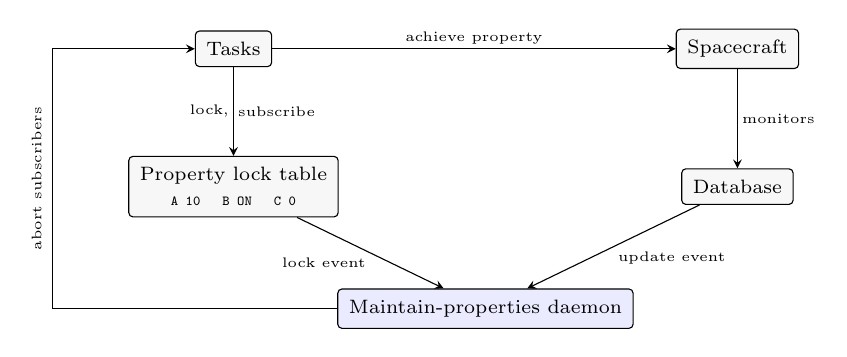
\begin{tikzpicture}[
  font=\scriptsize, >=stealth,
  box/.style={draw, rounded corners=1.5pt, align=center, inner sep=4pt,
              fill=black!3},
  lbl/.style={font=\tiny, inner sep=1.5pt}
]
  \node[box] (tasks) at (0,0)      {Tasks};
  \node[box] (sc)    at (6.4,0)    {Spacecraft};
  \node[box] (locks) at (0,-1.75)  {Property lock table\\[1pt]
        {\tiny\ttfamily A~10 \quad B~ON \quad C~0}};
  \node[box] (db)    at (6.4,-1.75) {Database};
  \node[box, fill=blue!8] (dae) at (3.2,-3.3) {Maintain-properties daemon};

  \draw[->] (tasks) -- node[lbl, above] {achieve property} (sc);
  \draw[->] (sc)    -- node[lbl, right] {monitors} (db);
  \draw[->] (tasks) -- node[lbl, left]  {lock,} node[lbl, right] {subscribe} (locks);
  \draw[->] (locks) -- node[lbl, below left]  {lock event}   (dae);
  \draw[->] (db)    -- node[lbl, below right] {update event} (dae);
  \draw[->] (dae.west) -- (-2.3,-3.3) -- (-2.3,0) -- (tasks.west);
  \node[lbl, rotate=90] at (-2.5,-1.65) {abort subscribers};
\end{tikzpicture}\par}

\pause
\vspace{0.2cm}

A task locks a property, then achieves it --- writing it into the spacecraft. The
{\bf database} is what the monitors actually observe. When the lock table says a
property is held and achieved but the database disagrees, that is an {\bf
inconsistency}, and the daemon must abort every task subscribed to it.

\end{frame}

%----------------------------------------
\begin{frame}[fragile]
  \frametitle{Two properties, written by the programmers} \small

Crucially, the RA programmers formulated these {\em after} the \promelaname{}
model had been written --- so the properties had no influence on the design of the
model, and the model was not built to satisfy them.

\vspace{0.25cm}

\begin{block}{RELEASE}\small
{\em A task releases all of its locks before it terminates.} \\
An assertion, placed after the task's body.
\end{block}

\pause

\begin{block}{ABORT}\small
{\em If an inconsistency occurs between the database and an entry in the lock
table, then all tasks that rely on the lock will be terminated.}
\begin{lstlisting}[language=promela]
[] (task1_property_broken -> <> task1_terminated)
\end{lstlisting}
A {\bf response} property --- the second of the three patterns from Part 3.
\end{block}

\pause
\vspace{0.2cm}

Both turned out to be broken. Five flawed code fragments: one breaking RELEASE,
three breaking ABORT, one efficiency bug. The programmer confirmed all five were
errors in the {\em Lisp}, not just in the model.

\end{frame}

%----------------------------------------
\begin{frame}[fragile]
  \frametitle{Error 2 --- the one that mattered} \small

Three counters:

\vspace{0.1cm}

{\scriptsize
\tool{Ev[MEMORY\_EVENT].count} --- how many times the database has changed.\\
\tool{Ev[LOCK\_EVENT].count} --- how many times the lock table has changed.\\
\tool{event\_count} --- the daemon's snapshot of their sum, last time it looked.\par}

\begin{lstlisting}[language=promela]
if                            /* has anything happened since I looked? */
:: (!first_time &&
    Ev[MEMORY_EVENT].count +
    Ev[LOCK_EVENT].count != event_count) ->
      event_count = Ev[MEMORY_EVENT].count +
                    Ev[LOCK_EVENT].count
:: else ->                    /* no: go to sleep */
      first_time = false;
      /* <-- an event arriving HERE is lost */
      wait_for_events(this, MEMORY_EVENT, LOCK_EVENT)
fi
\end{lstlisting}

\pause

The guard reads the event counters, the \ipromela{else} branch commits to
sleeping --- and the sleeping happens later, as a {\bf separate statement}.

\end{frame}

%----------------------------------------
\begin{frame}[fragile]
  \frametitle{Error 2 --- the fix} \small

\begin{lstlisting}[language=promela]
atomic {                      /* deciding and sleeping, indivisibly */
  if
  :: (!first_time && ...) -> event_count = ...
  :: else -> first_time = false;
             wait_for_events(this, MEMORY_EVENT, LOCK_EVENT)
  fi
}
\end{lstlisting}

\vspace{0.15cm}

One keyword. The daemon can no longer be preempted between deciding that nothing
has happened and going to sleep.

\pause
\vspace{0.3cm}

\begin{block}{}\small
{\em The same shape as the queue.} There it was publish-then-credit; here it is
check-then-wait. Both are a test and the act that depends on it, performed as two
steps --- and in both cases the whole bug is the gap between them.
\end{block}

\end{frame}

%----------------------------------------
\begin{frame}
  \frametitle{18 May 1999} \small

Deep Space 1, 96 million kilometres from Earth. {\bf Thrusting did not turn off
when requested.} The Remote Agent experiment was terminated from the ground and
the spacecraft put into stand-by mode.

\pause
\vspace{0.3cm}

The cause was a deadlock: a missing critical section around a conditional wait,
letting an event arrive between the evaluation of the condition and the wait. The
thread waited, missed the event, and the system wedged.

\pause
\vspace{0.3cm}

\begin{block}{}\small
{\bf The same defect as Error 2} --- and not by coincidence. The code had been
{\bf copied} into another module, and the critical section around it was, by
mistake, left out of the copy. That module was never analyzed with \spin{}.

\vspace{0.15cm}

The repair was to put the critical section back --- the fix \spin{}'s error trace
had already produced, months earlier, for the same pattern elsewhere.
\end{block}

\end{frame}

%----------------------------------------
\begin{frame}
  \frametitle{What the programmer said} \small

On Error 1:

\begin{block}{}\small
{\em ``This is a particularly pernicious bug. It arises only because you are in a
multi-threaded environment, and only in very obscure circumstances that are very
unlikely to arise during testing. Congratulations! You have just converted me into
a believer in formal methods.''}
\end{block}

\pause

On Error 2 --- the pattern that later flew:

\begin{block}{}\small
{\em ``This is an instance of a classic pattern: not wrapping a conditional
wait-for-events inside a critical section. This sort of mistake is very easy to
make and happens all the time in our code. Thanks for catching this one!''}
\end{block}

\pause

Afterwards:

\begin{block}{}\small
{\em ``I used to be very skeptical of the utility of formal methods\dots{} what you
have been doing is finding places where software violates design assumptions,
which is not the same thing as proving correctness. To me you have demonstrated
the utility of this approach beyond any question.''}
\end{block}

\end{frame}
